% Author @ Huyen Tran, DONE

%\subsection{Ford Fulkerson Method}
\label{ford-fulkerson method}
The Ford-Fulkerson method, introduced by L.R. Ford and D.R. Fulkerson in 1956, solves the maximum flow problem in a flow network, where the objective is to maximize the flow from a source $s$ to a sink $t$ through various paths in a network of directed edges with defined capacities. This method was originally inspired by real-world network problems, such as maximizing transport flow across a rail network, where each segment has a fixed capacity \cite{ford1956flows}. The Ford-Fulkerson method iteratively finds \textbf{augmenting paths} in the \textbf{residual network}, increasing the flow until no more augmenting paths exist. It operates based on three key concepts: \textbf{residual network}, \textbf{flow augmentation}, and the \textbf{max-flow min-cut theorem}.

\paragraph*{a. Residual Networks:}A residual network represents the capacities of edges that remain available for flow augmentation in a flow network. Given a flow network $G = (V, E)$ with a current flow $f$, the residual capacity $c_f(u, v)$  for any pair of vertices $(u, v)$ is formally defined as:
    \[
    c_f(u, v) =
    \begin{cases} 
    c(u, v) - f(u, v) & \text{if } (u, v) \in E, \\
    f(v, u) & \text{if } (v, u) \in E, \\
    0 & \text{otherwise}.
    \end{cases}
    \]
    \textbf{Forward edges} correspond to edges \( (u, v) \in E \), the residual capacity \( c_f(u, v) = c(u, v) - f(u, v) \),  where \( f(u, v) < c(u, v) \), indicates the remaining capacity that can accommodate additional flow. To allow reduction of flow along an edge, \( G_f \) also includes a \textbf{reverse edge} \( (v, u) \) with residual capacity \( c_f(v, u) = f(u, v) \) if $f(u,v) < c(u,v)$. These reverse edges enable flow cancellation, which is crucial for algorithms to correct or optimize the flow. Therefore, residual edges \( (u, v) \) exist in \( G_f \) if and only if \( c_f(u, v) > 0 \).
    
    \noindent The residual network $G_f$ includes residual edges, which either allow additional flow along edges of $G$ or enable the reduction of flow via reverse edges. This structure is central to finding augmenting paths that represent directions in which the flow in $G$ can be increased.\\
    For example, consider an edge $(u, v)$ with capacity \( c(u, v) = 16 \) and flow \( f(u, v) = 11 \): $c_f(u, v) = 16 - 11 = 5, c_f(v, u) = 11$. This allows adding up to 5 units of flow on $(u, v)$ or reducing it by up to 11 units via \( (v, u) \).

\paragraph*{b. Flow Augmentation:} Flow augmentation refers to increasing the total flow in the network by sending additional flow along an augmenting path in the residual network. An \textbf{augmenting path} in a flow network $G = (V, E)$ with a flow $f$ is a simple path from the source $s$ to the sink $t$ in the residual network $G_f$. Along this path, the flow can be increased on each edge without violating capacity constraints. For an augmenting path $p$, the \textbf{residual capacity} $c_f(p)$ is defined as:
\[
c_f(p) = \min \{ c_f(u, v) \mid (u, v) \text{ is on } p \}.
\]
\noindent This value represents the maximum flow that can be added to the edges along $p$ without exceeding their residual capacities. For example, if the smallest residual capacity along $p$ is $c_f(2, 3) = 4$, the flow can be increased by up to 4 units along the entire path. To augment the flow along $p$, a new flow function $f_p$ is defined as:
\[
f_p(u, v) =
\begin{cases} 
c_f(p) & \text{if } (u, v) \text{ is on } p, \\
0 & \text{otherwise}.
\end{cases}
\]
Here, $f_p$ represents the flow contributed by $p$, with a total value $|f_p| = c_f(p) > 0$.\\

\noindent The augmented flow $f \oplus f_p$ in the original network $G$ is obtained by adding $f_p$ to $f$:
\[
(f \oplus f_p)(u, v) = 
\begin{cases} 
f(u, v) + f_p(u, v) & \text{if } (u, v) \text{ is in } E, \\
f(u, v) - f_p(v, u) & \text{if } (v, u) \text{ is in } E, \\
0 & \text{otherwise}.
\end{cases}
\]
The augmented flow $f \oplus f_p$ in the original network $G$ is updated for each edge. For forward edges $(u, v)$, the flow increases by $c_f(p)$, reducing $c_f(u, v)$. For reverse edges $(v, u)$, the flow decreases by $c_f(p)$, increasing $c_f(v, u)$. These updates adjust the residual network $G_f$, enabling iterative improvements to the total flow. Each augmenting step ensures that the new flow remains valid in the network and increases the total flow by the value of $f_p$, bringing the solution closer to the maximum flow. 


\paragraph*{c. Max-Flow Min-Cut Theorem:} Building on the relationship between flows and cuts, the Max-Flow Min-Cut Theorem establishes a fundamental equivalence: the value of the maximum flow in a flow network equals the capacity of the minimum cut.

\noindent The value of the \textbf{maximum flow} from the source $s$ to the sink $t$ equals the total net flow across the network:
$f(S, T) = |f|$. A \textbf{cut} in a flow network $G = (V, E)$ is a partition of the vertex set $V$ into two disjoint subsets $S$ and $T = V \setminus S$, such that the source $s \in S$ and the sink $t \in T$. The net flow $f(S, T)$ across a cut $(S, T)$ is defined as:
\[
f(S, T) = \sum_{u \in S} \sum_{v \in T} f(u, v) - \sum_{u \in S} \sum_{v \in T} f(v, u).
\]
This accounts for the flow leaving $S$ and subtracts the flow entering $S$ from $T$. The capacity $c(S, T)$ of a cut is the sum of the capacities of edges crossing from $S$ to $T$:
\[
c(S, T) = \sum_{u \in S} \sum_{v \in T} c(u, v).
\]
Unlike flow, the capacity only considers edges directed from $S$ to $T$.

\noindent A \textbf{minimum cut} is the cut with the smallest capacity among all possible cuts of the network. Flow across a cut accounts for both directions (from $S$ to $T$ and $T$ to $S$), while capacity considers only edges directed from $S$ to $T$. For any flow $f$, the net flow across any cut equals the value of the flow, $|f|$, ensuring consistency across different cuts:$f(S, T) = |f|.$
\noindent Cuts provide an upper bound for the value of any flow since the flow cannot exceed the capacity of a cut. Among all cuts, the minimum cut's capacity matches the maximum flow in the network. The Max-Flow Min-Cut Theorem captures this duality:

\begin{theorem} {Max-Flow Min-Cut Theorem} \label{max-flow theorem}\\
If $f$ is a flow in a flow network $G = (V, E)$  with source $s$ and sink $t$, then the
following conditions are equivalent:\\
1. $f$ is a maximum flow in $G$.\\
2. The residual network $G_f$ contains no augmenting paths.\\
3. $|f| = c(S, T)$ for some cut $(S, T)$ of $G$.
\end{theorem}

\noindent The Theorem \ref{max-flow theorem} states that: A flow $f$ is a maximum flow if and only if the residual network $G_f$ contains no augmenting paths and The value of the maximum flow equals the capacity of the minimum cut: $|f| = c(S, T)$ for some minimum cut $(S, T)$.

\paragraph{Ford-Fulkerson Basic Algorithm:}
The Ford-Fulkerson algorithm iteratively solves the maximum flow problem by leveraging the residual network $G_f$. At each step, it identifies an augmenting path $p$ from the source $s$ to the sink $t$ and augments the flow $f$ along $p$ by the residual capacity $c_f(p)$, defined as the minimum residual capacity of all edges in $p$
\begin{codebox}
\Procname{\proc{Ford-Fulkerson}$(G, s, t)$}
\li \For each edge $(u, v) \in E$ \Do
\li \quad $f(u,v) = 0$
    \End
\li \While there exists a path $p$ from $s$ to $t$ in the residual network $G_f$ \Do
\li \quad $c_f(p)$ = min($c_f(u,v):(u,v)$ is in $p$)
\li \quad \For each edge $(u, v)$ is in $p$ \Do
\li \quad \If $(u, v) \in E$ \Do
\li \quad  $f(u,v) = f(u,v) + c_f(p) $
\li \quad \Else $f(v,u) = f(v,u) - c_f(p) $
          \End
    \End
\end{codebox}

% First graph
\begin{figure}[ht]
\centering

% First row: (a) and the first graph
\begin{subfigure}[t]{0.45\textwidth}
\centering
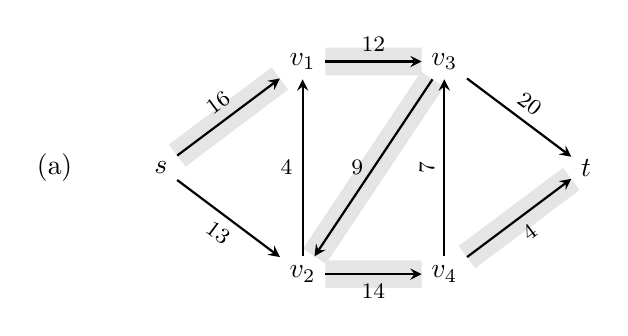
\begin{tikzpicture}[>=stealth, scale=0.9]
    % Nodes for graph (a)
    \node at (-1.5, 0) {(a)}; % Label for graph (a)
    \node (s) at (0, 0) {$s$};
    \node (v1) at (2, 1.5) {$v_1$};
    \node (v2) at (2, -1.5) {$v_2$};
    \node (v3) at (4, 1.5) {$v_3$};
    \node (v4) at (4, -1.5) {$v_4$};
    \node (t) at (6, 0) {$t$};

    % Highlighted augmenting path
    \draw[gray!20, line width=10pt, rounded corners] 
    (s) -- (v1) -- (v3) -- (v2) -- (v4) -- (t);
    
    % Edges with capacities
    \draw[->, thick] (s) -- (v1) node[midway, above, sloped, font=\footnotesize] {16};
    \draw[->, thick] (s) -- (v2) node[midway, below, sloped, font=\footnotesize] {13};
    \draw[->, thick] (v1) -- (v3) node[midway, above, sloped, font=\footnotesize] {12};
    \draw[->, thick] (v2) -- (v1) node[midway, left, font=\footnotesize] {4};
    \draw[->, thick] (v2) -- (v4) node[midway, below, sloped, font=\footnotesize] {14};
    \draw[->, thick] (v3) -- (v2) node[midway, left, font=\footnotesize] {9};
    \draw[->, thick] (v3) -- (t) node[midway, above, sloped, font=\footnotesize] {20};
    \draw[->, thick] (v4) -- (v3) node[midway, above, sloped, font=\footnotesize] {7};
    \draw[->, thick] (v4) -- (t) node[midway, below, sloped, font=\footnotesize] {4};
\end{tikzpicture}
\end{subfigure}
\hfill
\begin{subfigure}[t]{0.45\textwidth}
\centering
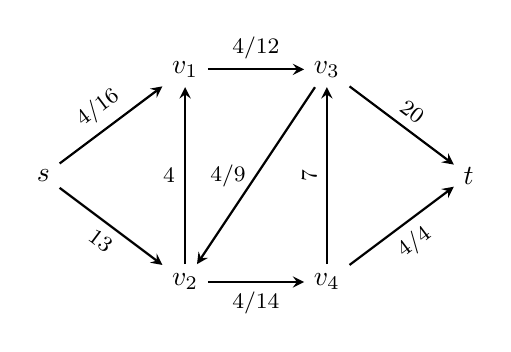
\begin{tikzpicture}[>=stealth, scale=0.9]
    % Nodes for the first graph on the right
    \node (s) at (0, 0) {$s$};
    \node (v1) at (2, 1.5) {$v_1$};
    \node (v2) at (2, -1.5) {$v_2$};
    \node (v3) at (4, 1.5) {$v_3$};
    \node (v4) at (4, -1.5) {$v_4$};
    \node (t) at (6, 0) {$t$};

    % Edges with flows/capacities
    \draw[->, thick] (s) -- (v1) node[midway, above, sloped, font=\footnotesize] {4/16};
    \draw[->, thick] (s) -- (v2) node[midway, below, sloped, font=\footnotesize] {13};
    \draw[->, thick] (v1) -- (v3) node[midway, above, sloped, font=\footnotesize] {4/12};
    \draw[->, thick] (v2) -- (v1) node[midway, left, font=\footnotesize] {4};
    \draw[->, thick] (v2) -- (v4) node[midway, below, sloped, font=\footnotesize] {4/14};
    \draw[->, thick] (v3) -- (v2) node[midway, left, font=\footnotesize] {4/9};
    \draw[->, thick] (v3) -- (t) node[midway, above, sloped, font=\footnotesize] {20};
    \draw[->, thick] (v4) -- (v3) node[midway, above, sloped, font=\footnotesize] {7};
    \draw[->, thick] (v4) -- (t) node[midway, below, sloped, font=\footnotesize] {4/4};
\end{tikzpicture}
\end{subfigure}

\vspace{0.25cm}

% Second row: (b) and the second graph
\begin{subfigure}[t]{0.45\textwidth}
\centering
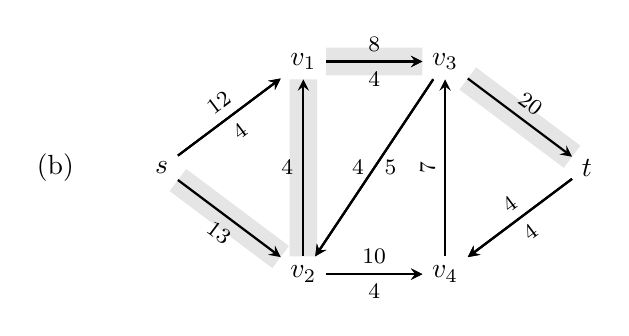
\begin{tikzpicture}[>=stealth, scale=0.9]
    % Nodes for graph (b)
    \node at (-1.5, 0) {(b)}; % Label for graph (b)
    \node (s) at (0, 0) {$s$};
    \node (v1) at (2, 1.5) {$v_1$};
    \node (v2) at (2, -1.5) {$v_2$};
    \node (v3) at (4, 1.5) {$v_3$};
    \node (v4) at (4, -1.5) {$v_4$};
    \node (t) at (6, 0) {$t$};

    % Highlighted augmenting path
    \draw[gray!20, line width=10pt, rounded corners] 
    (s) -- (v2) -- (v1) -- (v3) -- (t);

    % Forward Edges with capacities
    \draw[->, thick] (s) -- (v1) node[midway, above, sloped, font=\footnotesize] {12};
    \draw[->, thick] (s) -- (v2) node[midway, below, sloped, font=\footnotesize] {13};
    \draw[->, thick] (v1) -- (v3) node[midway, above, sloped, font=\footnotesize] {8};
    \draw[->, thick] (v2) -- (v1) node[midway, left, font=\footnotesize] {4};
    \draw[->, thick] (v2) -- (v4) node[midway, above, sloped, font=\footnotesize] {10};
    \draw[->, thick] (v3) -- (v2) node[midway, right, font=\footnotesize] {5};
    \draw[->, thick] (v3) -- (t) node[midway, above, sloped, font=\footnotesize] {20};
    \draw[->, thick] (v4) -- (v3) node[midway, above, sloped, font=\footnotesize] {7};
    \draw[<-, thick] (v4) -- (t) node[midway, below, sloped, font=\footnotesize] {4};

    % Reverse Edges with reverse capacities
    \draw[<-, thick] (v1) -- (s) node[midway, below, sloped, font=\footnotesize] {4};
    \draw[<-, thick] (v3) -- (v1) node[midway, below, sloped, font=\footnotesize] {4};
    \draw[<-, thick] (v2) -- (v3) node[midway, left, font=\footnotesize] {4};
    \draw[<-, thick] (v4) -- (v2) node[midway, below, sloped, font=\footnotesize] {4};
    \draw[->, thick] (t) -- (v4) node[midway, above, sloped, font=\footnotesize] {4};
\end{tikzpicture}
\end{subfigure}
\hfill
\begin{subfigure}[t]{0.45\textwidth}
\centering
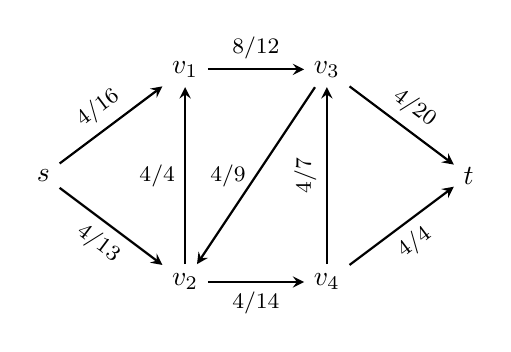
\begin{tikzpicture}[>=stealth, scale=0.9]
    % Nodes for the second graph on the right
    \node (s) at (0, 0) {$s$};
    \node (v1) at (2, 1.5) {$v_1$};
    \node (v2) at (2, -1.5) {$v_2$};
    \node (v3) at (4, 1.5) {$v_3$};
    \node (v4) at (4, -1.5) {$v_4$};
    \node (t) at (6, 0) {$t$};

    % Edges with flows/capacities
    \draw[->, thick] (s) -- (v1) node[midway, above, sloped, font=\footnotesize] {4/16};
    \draw[->, thick] (s) -- (v2) node[midway, below, sloped, font=\footnotesize] {4/13};
    \draw[->, thick] (v1) -- (v3) node[midway, above, sloped, font=\footnotesize] {8/12};
    \draw[->, thick] (v2) -- (v1) node[midway, left, font=\footnotesize] {4/4};
    \draw[->, thick] (v2) -- (v4) node[midway, below, sloped, font=\footnotesize] {4/14};
    \draw[->, thick] (v3) -- (v2) node[midway, left, font=\footnotesize] {4/9};
    \draw[->, thick] (v3) -- (t) node[midway, above, sloped, font=\footnotesize] {4/20};
    \draw[->, thick] (v4) -- (v3) node[midway, above, sloped, font=\footnotesize] {4/7};
    \draw[->, thick] (v4) -- (t) node[midway, below, sloped, font=\footnotesize] {4/4};
\end{tikzpicture}
\end{subfigure}

\vspace{0.25cm}

% Third row: (c) and the second graph
\begin{subfigure}[t]{0.45\textwidth}
\centering
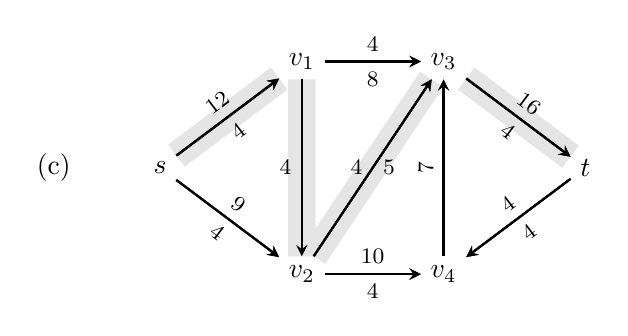
\begin{tikzpicture}[>=stealth, scale=0.9]
    % Nodes for graph (b)
    \node at (-1.5, 0) {(c)}; % Label for graph (c)
    \node (s) at (0, 0) {$s$};
    \node (v1) at (2, 1.5) {$v_1$};
    \node (v2) at (2, -1.5) {$v_2$};
    \node (v3) at (4, 1.5) {$v_3$};
    \node (v4) at (4, -1.5) {$v_4$};
    \node (t) at (6, 0) {$t$};

    % Highlighted augmenting path
    \draw[gray!20, line width=10pt, rounded corners] 
    (s) -- (v1) -- (v2) -- (v3) -- (t);

    % Forward Edges with capacities
    \draw[->, thick] (s) -- (v1) node[midway, above, sloped, font=\footnotesize] {12};
    \draw[->, thick] (s) -- (v2) node[midway, above, sloped, font=\footnotesize] {9};
    \draw[->, thick] (v1) -- (v3) node[midway, above, sloped, font=\footnotesize] {4};
    \draw[->, thick] (v1) -- (v2) node[midway, left, font=\footnotesize] {4};
    \draw[->, thick] (v2) -- (v4) node[midway, above, sloped, font=\footnotesize] {10};
    \draw[->, thick] (v2) -- (v3) node[midway, right, font=\footnotesize] {5};
    \draw[->, thick] (v3) -- (t) node[midway, above, sloped, font=\footnotesize] {16};
    \draw[->, thick] (v4) -- (v3) node[midway, above, sloped, font=\footnotesize] {7};
    \draw[->, thick] (t) -- (v4) node[midway, below, sloped, font=\footnotesize] {4};

     % Reverse Edges with reverse capacities
    \draw[<-, thick] (v1) -- (s) node[midway, below, sloped, font=\footnotesize] {4};
    \draw[<-, thick] (v2) -- (s) node[midway, below, sloped, font=\footnotesize] {4};
    \draw[<-, thick] (v3) -- (v1) node[midway, below, sloped, font=\footnotesize] {8};
    \draw[->, thick] (v2) -- (v3) node[midway, left, font=\footnotesize] {4};
    \draw[<-, thick] (v4) -- (v2) node[midway, below, sloped, font=\footnotesize] {4};
    \draw[->, thick] (t) -- (v4) node[midway, above, sloped, font=\footnotesize] {4};
    \draw[<-, thick] (t) -- (v3) node[midway, below, sloped, font=\footnotesize] {4};
\end{tikzpicture}
\end{subfigure}
\hfill
\begin{subfigure}[t]{0.45\textwidth}
\centering
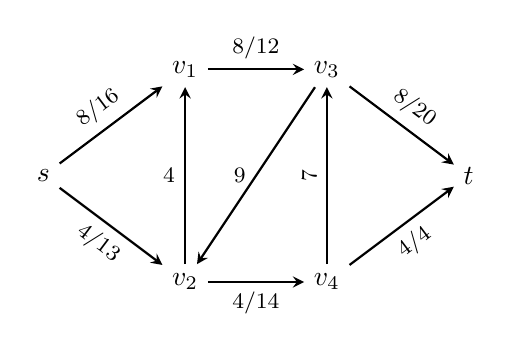
\begin{tikzpicture}[>=stealth, scale=0.9]
    % Nodes for the second graph on the right
    \node (s) at (0, 0) {$s$};
    \node (v1) at (2, 1.5) {$v_1$};
    \node (v2) at (2, -1.5) {$v_2$};
    \node (v3) at (4, 1.5) {$v_3$};
    \node (v4) at (4, -1.5) {$v_4$};
    \node (t) at (6, 0) {$t$};

    % Edges with flows/capacities
    \draw[->, thick] (s) -- (v1) node[midway, above, sloped, font=\footnotesize] {8/16};
    \draw[->, thick] (s) -- (v2) node[midway, below, sloped, font=\footnotesize] {4/13};
    \draw[->, thick] (v1) -- (v3) node[midway, above, sloped, font=\footnotesize] {8/12};
    \draw[->, thick] (v2) -- (v1) node[midway, left, font=\footnotesize] {4};
    \draw[->, thick] (v2) -- (v4) node[midway, below, sloped, font=\footnotesize] {4/14};
    \draw[->, thick] (v3) -- (v2) node[midway, left, font=\footnotesize] {9};
    \draw[->, thick] (v3) -- (t) node[midway, above, sloped, font=\footnotesize] {8/20};
    \draw[->, thick] (v4) -- (v3) node[midway, above, sloped, font=\footnotesize] {7};
    \draw[->, thick] (v4) -- (t) node[midway, below, sloped, font=\footnotesize] {4/4};
\end{tikzpicture}
\end{subfigure}

\caption{The execution of the basic Ford-Fulkerson algorithm. (a)–(e) Successive iterations of
the while loop. The left side of each part shows the residual network Gf from line 3 with a shaded
augmenting path p. The right side of each part shows the new flow f that results from augmenting f
by fp. The residual network in (a) is the input network G. The residual capacity $c_f$ is above/ on the left of each forward edge and is below/on the right of its reverse edge.}
\label{ff_graph(1)}
\end{figure}

\noindent The algorithm operates as follows:
\begin{enumerate}
    \item \textbf{Initialization:} Set $f(u, v) = 0$ for all edges $(u, v) \in E$.
    \item \textbf{Residual Network and Augmenting Paths:} 
    \begin{itemize}
        \item The algorithm operates on a residual network $G_f$, which represents how much additional flow can be pushed along each edge.
        \item For each edge $(u,v)$, the residual capacity $c_f(u,v)$ is calculated based on the edge’s capacity minus the current flow. 
        \item If a path from $s$ to $t$ exists in the residual network $G_f$ (with positive residual capacity on each edge), this path is called an augmenting path.
    \end{itemize}
    \item \textbf{Flow Augmentation:} 
    \begin{itemize}
        \item For each augmenting path $p$, determine the bottleneck capacity $c_f(p)$, which is the minimum residual capacity along that path.
        \item Increase the flow $f$ along the path $p$ by the residual capacity. Update the flow and residual capacities for each edge: If the edge is in the original direction, add the residual capacity to the flow. If the edge is in the reverse direction, subtract the residual capacity from the flow.
    \end{itemize}
    \item \textbf{Termination:} Repeat the process until there are no more augmenting paths in the residual network. When no augmenting paths are left, the flow $f$ represents the maximum flow from $s$ to $t$.
\end{enumerate}
The termination of the algorithm is validated by theorem \ref{max-flow theorem}, which states that a flow is maximized if and only if there are no augmenting paths left in the residual network.

%Second graph
\begin{figure}[ht]
\centering

% First row: (d) and the first graph
\begin{subfigure}[t]{0.45\textwidth}
\centering
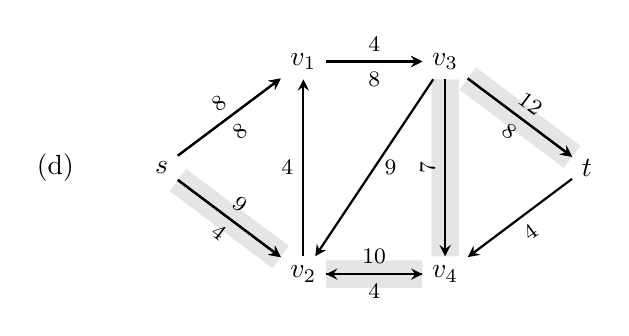
\begin{tikzpicture}[>=stealth, scale=0.9]
    % Nodes for graph (d)
    \node at (-1.5, 0) {(d)}; % Label for graph (a)
    \node (s) at (0, 0) {$s$};
    \node (v1) at (2, 1.5) {$v_1$};
    \node (v2) at (2, -1.5) {$v_2$};
    \node (v3) at (4, 1.5) {$v_3$};
    \node (v4) at (4, -1.5) {$v_4$};
    \node (t) at (6, 0) {$t$};

    % Highlighted augmenting path
    \draw[gray!20, line width=10pt, rounded corners] 
    (s) -- (v2) -- (v4) -- (v3) -- (t);
    
    % Edges with capacities
    \draw[->, thick] (s) -- (v1) node[midway, above, sloped, font=\footnotesize] {8};
    \draw[<-, thick] (v1) -- (s) node[midway, below, sloped, font=\footnotesize] {8};
    \draw[->, thick] (s) -- (v2) node[midway, above, sloped, font=\footnotesize] {9};
    \draw[->, thick] (s) -- (v2) node[midway, below, sloped, font=\footnotesize] {4};
    \draw[->, thick] (v1) -- (v3) node[midway, above, sloped, font=\footnotesize] {4};
    \draw[->, thick] (v1) -- (v3) node[midway, below, sloped, font=\footnotesize] {8};
    \draw[<-, thick] (v1) -- (v2) node[midway, left, font=\footnotesize] {4};
    \draw[->, thick] (v2) -- (v4) node[midway, above, sloped, font=\footnotesize] {10};
    \draw[<-, thick] (v2) -- (v4) node[midway, below, sloped, font=\footnotesize] {4};
    \draw[<-, thick] (v2) -- (v3) node[midway, right, font=\footnotesize] {9};
    \draw[->, thick] (v3) -- (t) node[midway, above, sloped, font=\footnotesize] {12};
    \draw[->, thick] (v3) -- (t) node[midway, below, sloped, font=\footnotesize] {8};
    \draw[<-, thick] (v4) -- (v3) node[midway, above, sloped, font=\footnotesize] {7};
    \draw[->, thick] (t) -- (v4) node[midway, below, sloped, font=\footnotesize] {4};
\end{tikzpicture}
\end{subfigure}
\hfill
\begin{subfigure}[t]{0.45\textwidth}
\centering
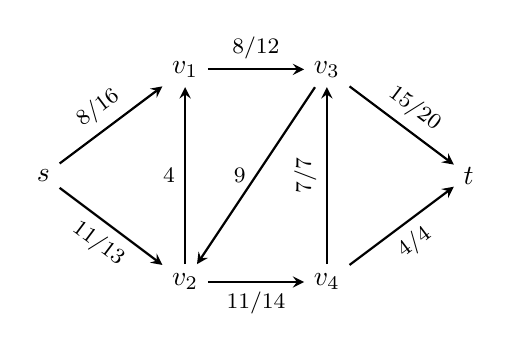
\begin{tikzpicture}[>=stealth, scale=0.9]
    % Nodes for the first graph on the right
    \node (s) at (0, 0) {$s$};
    \node (v1) at (2, 1.5) {$v_1$};
    \node (v2) at (2, -1.5) {$v_2$};
    \node (v3) at (4, 1.5) {$v_3$};
    \node (v4) at (4, -1.5) {$v_4$};
    \node (t) at (6, 0) {$t$};

    % Edges with flows/capacities
    \draw[->, thick] (s) -- (v1) node[midway, above, sloped, font=\footnotesize] {8/16};
    \draw[->, thick] (s) -- (v2) node[midway, below, sloped, font=\footnotesize] {11/13};
    \draw[->, thick] (v1) -- (v3) node[midway, above, sloped, font=\footnotesize] {8/12};
    \draw[->, thick] (v2) -- (v1) node[midway, left, font=\footnotesize] {4};
    \draw[->, thick] (v2) -- (v4) node[midway, below, sloped, font=\footnotesize] {11/14};
    \draw[->, thick] (v3) -- (v2) node[midway, left, font=\footnotesize] {9};
    \draw[->, thick] (v3) -- (t) node[midway, above, sloped, font=\footnotesize] {15/20};
    \draw[->, thick] (v4) -- (v3) node[midway, above, sloped, font=\footnotesize] {7/7};
    \draw[->, thick] (v4) -- (t) node[midway, below, sloped, font=\footnotesize] {4/4};
\end{tikzpicture}
\end{subfigure}

\vspace{0.25cm}

% Second row: (e) and the second graph
\begin{subfigure}[t]{0.45\textwidth}
\centering
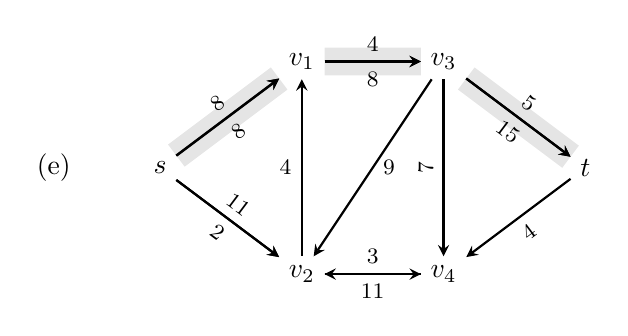
\begin{tikzpicture}[>=stealth, scale=0.9]
    % Nodes for graph (e)
    \node at (-1.5, 0) {(e)}; % Label for graph (e)
    \node (s) at (0, 0) {$s$};
    \node (v1) at (2, 1.5) {$v_1$};
    \node (v2) at (2, -1.5) {$v_2$};
    \node (v3) at (4, 1.5) {$v_3$};
    \node (v4) at (4, -1.5) {$v_4$};
    \node (t) at (6, 0) {$t$};

    % Highlighted augmenting path
    \draw[gray!20, line width=10pt, rounded corners] 
    (s) -- (v1) -- (v3) -- (t);

    % Edges with capacities
    \draw[->, thick] (s) -- (v1) node[midway, above, sloped, font=\footnotesize] {8};
    \draw[<-, thick] (v1) -- (s) node[midway, below, sloped, font=\footnotesize] {8};
    \draw[->, thick] (s) -- (v2) node[midway, above, sloped, font=\footnotesize] {11};
    \draw[->, thick] (s) -- (v2) node[midway, below, sloped, font=\footnotesize] {2};
    \draw[->, thick] (v1) -- (v3) node[midway, above, sloped, font=\footnotesize] {4};
    \draw[->, thick] (v1) -- (v3) node[midway, below, sloped, font=\footnotesize] {8};
    \draw[<-, thick] (v1) -- (v2) node[midway, left, font=\footnotesize] {4};
    \draw[->, thick] (v2) -- (v4) node[midway, above, sloped, font=\footnotesize] {3};
    \draw[<-, thick] (v2) -- (v4) node[midway, below, sloped, font=\footnotesize] {11};
    \draw[<-, thick] (v2) -- (v3) node[midway, right, font=\footnotesize] {9};
    \draw[->, thick] (v3) -- (t) node[midway, above, sloped, font=\footnotesize] {5};
    \draw[->, thick] (v3) -- (t) node[midway, below, sloped, font=\footnotesize] {15};
    \draw[<-, thick] (v4) -- (v3) node[midway, above, sloped, font=\footnotesize] {7};
    \draw[->, thick] (t) -- (v4) node[midway, below, sloped, font=\footnotesize] {4};
\end{tikzpicture}
\end{subfigure}
\hfill
\begin{subfigure}[t]{0.45\textwidth}
\centering
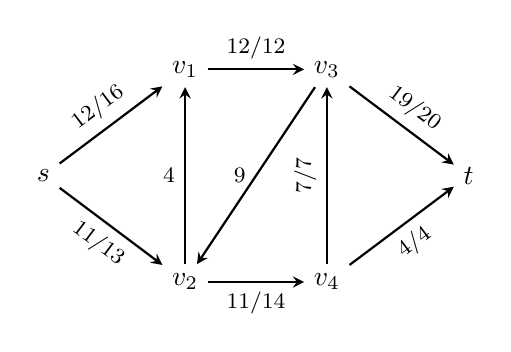
\begin{tikzpicture}[>=stealth, scale=0.9]
    % Nodes for the second graph on the right
    \node (s) at (0, 0) {$s$};
    \node (v1) at (2, 1.5) {$v_1$};
    \node (v2) at (2, -1.5) {$v_2$};
    \node (v3) at (4, 1.5) {$v_3$};
    \node (v4) at (4, -1.5) {$v_4$};
    \node (t) at (6, 0) {$t$};

    % Edges with flows/capacities
    \draw[->, thick] (s) -- (v1) node[midway, above, sloped, font=\footnotesize] {12/16};
    \draw[->, thick] (s) -- (v2) node[midway, below, sloped, font=\footnotesize] {11/13};
    \draw[->, thick] (v1) -- (v3) node[midway, above, sloped, font=\footnotesize] {12/12};
    \draw[->, thick] (v2) -- (v1) node[midway, left, font=\footnotesize] {4};
    \draw[->, thick] (v2) -- (v4) node[midway, below, sloped, font=\footnotesize] {11/14};
    \draw[->, thick] (v3) -- (v2) node[midway, left, font=\footnotesize] {9};
    \draw[->, thick] (v3) -- (t) node[midway, above, sloped, font=\footnotesize] {19/20};
    \draw[->, thick] (v4) -- (v3) node[midway, above, sloped, font=\footnotesize] {7/7};
    \draw[->, thick] (v4) -- (t) node[midway, below, sloped, font=\footnotesize] {4/4};
\end{tikzpicture}
\end{subfigure}

\vspace{0.25cm}

% Third row: (f) 
\begin{subfigure}[t]{0.45\textwidth}
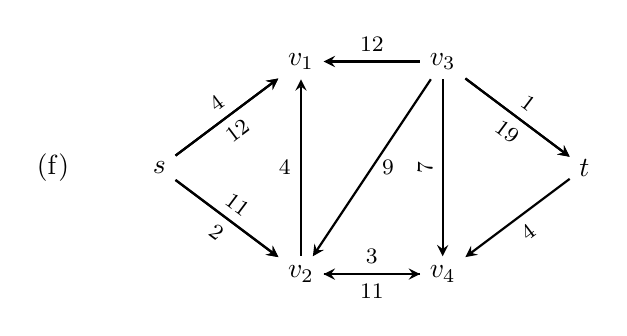
\begin{tikzpicture}[>=stealth, scale=0.9]
    % Nodes for graph (f)
    \node at (-1.5, 0) {(f)}; % Label for graph (f)
    \node (s) at (0, 0) {$s$};
    \node (v1) at (2, 1.5) {$v_1$};
    \node (v2) at (2, -1.5) {$v_2$};
    \node (v3) at (4, 1.5) {$v_3$};
    \node (v4) at (4, -1.5) {$v_4$};
    \node (t) at (6, 0) {$t$};

    % Forward Edges with capacities
    \draw[->, thick] (s) -- (v1) node[midway, above, sloped, font=\footnotesize] {4};
    \draw[<-, thick] (v1) -- (s) node[midway, below, sloped, font=\footnotesize] {12};
    \draw[->, thick] (s) -- (v2) node[midway, above, sloped, font=\footnotesize] {11};
    \draw[->, thick] (s) -- (v2) node[midway, below, sloped, font=\footnotesize] {2};
    \draw[<-, thick] (v1) -- (v3) node[midway, above, sloped, font=\footnotesize] {12};
    \draw[<-, thick] (v1) -- (v2) node[midway, left, font=\footnotesize] {4};
    \draw[->, thick] (v2) -- (v4) node[midway, above, sloped, font=\footnotesize] {3};
    \draw[<-, thick] (v2) -- (v4) node[midway, below, sloped, font=\footnotesize] {11};
    \draw[<-, thick] (v2) -- (v3) node[midway, right, font=\footnotesize] {9};
    \draw[->, thick] (v3) -- (t) node[midway, above, sloped, font=\footnotesize] {1};
    \draw[->, thick] (v3) -- (t) node[midway, below, sloped, font=\footnotesize] {19};
    \draw[<-, thick] (v4) -- (v3) node[midway, above, sloped, font=\footnotesize] {7};
    \draw[->, thick] (t) -- (v4) node[midway, below, sloped, font=\footnotesize] {4};
\end{tikzpicture}
\end{subfigure}
\caption{\textbf{(f)} The residual network at the last while loop test. It has no augmenting
paths and the flow $f$ shown in (e) is therefore a maximum flow. The value of the maximum flow
found is 23}
\label{ff_graph(2)}
\end{figure}

% Example 
\paragraph{Example:} Given a graph with the residual network (a) from Figure \ref{ff_graph(1)}. We can go through the Ford-Fulkerson algorithm to find the maximum flow showed in (e) from Figure \ref{ff_graph(2)}:\\
\textbf{Initialization}: Set $f(u, v) = 0$ for all edges $(u, v) \in E$. The initial flow in the network is zero, and the residual capacities are equal to the original capacities.\\
\textbf{Residual Network and Augmenting Paths:} The algorithm constructs a residual network $G_f$, where each edge $(u, v)$ has a residual capacity:$c_f(u, v) = c(u, v) - f(u, v)$. Paths in $G_f$ with positive residual capacities are called augmenting paths. The augmenting paths for the example are as follows:
\par Path 1: $p1: s \to v_1 \to v_3 \to v_2 \to v_4 \to t$, residual capacity:
\par \quad $ c_f(p1)$ = $min(c_f(s,v1), c_f(v1,v3), c_f(v3,v2), c_f(v2,v4), c_f(v4,t))$ = $min(16, 12, 9, 14, 4)=4$.
\par Path 2: $p2: s \to v_2 \to v_1 \to v_3 \to t$, \quad $c_f(p2)=4$.
\par Path 3: $p3: s \to v_1 \to v_2 \to v_3 \to t$, \quad $c_f(p3)=4$.
\par Path 4: $p4: s \to v_2 \to v_4 \to v_3 \to t$, \quad $c_f(p4)=7$.
\par Path 5: $p5: s \to v_1 \to v_3 \to t$, \quad $c_f(p5)=4$.
\\
\textbf{Flow Augmentation:} For each augmenting path $p$, the flow $f$ is increased by the residual capacity $c_f(p)$. After each augmentation, the residual network $G_f$ is updated as follows:

\par Path 1: $s \to v_1 \to v_3 \to v_2 \to v_4 \to t$. The residual capacity $c_f(p) = 4$. 
\par \quad Flow Update: $f(s, v_1) = 4$, $f(v_1, v_3) = 4$, $f(v_3, v_2) = 4$, $f(v_2, v_4) = 4$, $f(v_4, t) = 4$.
\par \quad Residual update:
\par\quad Forward edges: $c_f(s, v_1) = 16 - 4 = 12, \quad c_f(v_1, v_3) = 12 - 4 = 8, \quad c_f(v_3, v_2) = 9 - 4 = 5, \quad c_f(v_2, v_4) = 14 - 4 = 10, \quad c_f(v_4, t) = 4 - 4 = 0$.
\par \quad Reverse edges: $ c_f(v_1, s) = 4, \quad c_f(v_3, v_1) = 4, \quad c_f(v_2, v_3) = 4, \quad c_f(v_4, v_2) = 4, \quad c_f(t, v_4) = 4$.

\par Path 2: $s \to v_2 \to v_1 \to v_3 \to t$. The residual capacity $c_f(p) = 4$. 
\par \quad Flow Update: $f(s, v_2) = 4, \quad f(v_2, v_1) = 4, \quad f(v_1, v_3) = 8, \quad f(v_3, t) = 4.$.
\par \quad Residual update: 
\par \quad Forward edges: $c_f(s, v_2) = 13 - 4 = 9, \quad c_f(v_2, v_1) = 4 - 4 = 0, \quad c_f(v_1, v_3) = 8 - 4 = 4, \quad c_f(v_3, t) = 20 - 4 = 16$.
\par \quad Reverse edges: $c_f(v_2, s) = 4, \quad c_f(v_1, v_2) = 4, \quad c_f(v_3, v_1) = 8, \quad c_f(t, v_3) = 4$.

\par Path 3: $s \to v_1 \to v_2 \to v_3 \to t$. The residual capacity $c_f(p) = 4$. 
\par \quad Flow Update: $f(s, v_1) = 8$, $f(v_1, v_2) = 4$, $f(v_2, v_3) = 4$, $f(v_3, t) = 8$.
\par \quad Forward edges: $c_f(s, v_1) = 12 - 4 = 8, \quad c_f(v_1, v_2) = 4 - 4 = 0, \quad c_f(v_2, v_3) = 10 - 4 = 6, \quad c_f(v_3, t) = 16 - 4 = 12$.
\par \quad Reverse edges: $c_f(v_1, s) = 4, \quad c_f(v_2, v_1) = 4, \quad c_f(v_3, v_2) = 4, \quad c_f(t, v_3) = 8$.

\par Path 4: $s \to v_2 \to v_4 \to v_3 \to t$. The residual capacity $c_f(p) = 7$. 
\par \quad Flow Update: $f(s, v_2) = 11$, $f(v_2, v_4) = 11$, $f(v_4, v_3) = 7$, $f(v_3, t) = 15$.
\par \quad Forward edges: $c_f(s, v_2) = 9 - 7 = 2, \quad c_f(v_2, v_4) = 10 - 7 = 3, \quad c_f(v_4, v_3) = 7 - 7 = 0, \quad c_f(v_3, t) = 12 - 7 = 5$.
\par \quad Reverse edges: $c_f(v_2, s) = 7, \quad c_f(v_4, v_2) = 7, \quad c_f(v_3, v_4) = 7, \quad c_f(t, v_3) = 7$.

\par Path 5: $s \to v_1 \to v_3 \to t$. The residual capacity $c_f(p) = 4$. Update:
$f(s, v_1) = 12$, $f(v_1, v_3) = 12$, $f(v_3, t) = 19$.
\par \quad Forward edges: $c_f(s, v_1) = 8 - 4 = 4, \quad c_f(v_1, v_3) = 4 - 4 = 0, \quad c_f(v_3, t) = 5 - 4 = 1$.
\par \quad Reverse edges: $c_f(v_1, s) = 4, \quad c_f(v_3, v_1) = 4, \quad c_f(t, v_3) = 4$.

\textbf{Termination:} When no more augmenting paths exist in the residual network $G_f$, the algorithm terminates. The final flow $f$ is: $f(s, v_1) = 12, \quad f(s, v_2) = 11, \quad f(v_1, v_3) = 12, \quad f(v_2, v_4) = 11, \quad f(v_4, v_3) = 7, \quad f(v_3, t) = 19$. The maximum flow is the total flow out of $s$, which is: $|f| = f(s, v_1) + f(s, v_2) = 12 + 11 = 23$.


\paragraph{Performance and Time Complexity}
The Ford-Fulkerson method has a time complexity of $O(E \cdot F)$ where $E$ is the number of edges and 
$F$ is the maximum possible flow in the network. For networks with integer capacities, the algorithm guarantees termination in finite steps, though in cases with irrational capacities, it may not converge. 


